\documentclass[tikz,border=12pt]{standalone}
% Shared visual language for standalone EMT block diagrams.
\usepackage{amsmath}
\usetikzlibrary{arrows.meta,backgrounds,calc,fit,positioning}

\tikzset{
    emt diagram/.style = {>={Stealth[length=2.4mm]}},
    line/.style        = {semithick, rounded corners=6pt},
    block/.style       = {draw, semithick, fill=white,
                          minimum height=1cm, minimum width=2.3cm},
    hblock/.style      = {block, minimum width=2.24cm, minimum height=1.3cm},
    vblock/.style      = {block, minimum width=1.3cm, minimum height=2.24cm},
    sum/.style         = {draw, semithick, fill=white, circle,
                          inner sep=2.6pt},
    signal/.style      = {circle, fill, inner sep=1.4pt,
                          label distance=3pt},
    sig/.style         = {font=\small},
    pm/.style          = {font=\scriptsize},
    wire jump/.style   = {line,
                          preaction={draw=white, line width=3pt,
                                     line cap=round}},
    enclosure/.style   = {draw, dashed, semithick, rounded corners=4pt},
    operator enclosure/.style = {enclosure, inner xsep=7mm, inner ysep=6mm}
}


\begin{document}
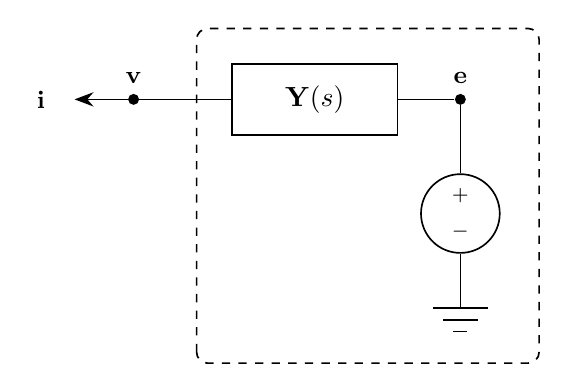
\begin{tikzpicture}[emt diagram]

% ================= Terminal admittance branch =================
\node[block, minimum width=2.1cm, minimum height=0.9cm]
    (Y) at (0, 1.15) {$\mathbf{Y}(s)$};

% ================= Terminal voltage and current =================
\node[signal, label={[sig]above:$\mathbf{v}$}] (vport) at (-2.3, 1.15) {};
\draw[->, line] (Y.west) -- (-3.05, 1.15);
\node[sig, anchor=east] at (-3.3, 1.15) {$\mathbf{i}$};

% ================= Internal source voltage =================
\node[signal, label={[sig]above:$\mathbf{e}$}] (enode) at (1.85, 1.15) {};
\draw[line] (Y.east) -- (enode);

% ================= Independent voltage source =================
\node[draw, semithick, fill=white, circle, minimum size=1.0cm]
    (source) at (1.85, -0.3) {};
\draw[line] (enode) -- (source.north);
\node[pm] at ($(source.center)+(0,0.23)$) {$+$};
\node[pm] at ($(source.center)+(0,-0.23)$) {$-$};

% ================= Ground reference =================
\draw[line] (source.south) -- (1.85, -1.50);
\draw[semithick] (1.50, -1.50) -- (2.20, -1.50);
\draw[semithick] (1.63, -1.65) -- (2.07, -1.65);
\draw[semithick] (1.76, -1.80) -- (1.94, -1.80);

% ================= Model enclosure =================
\draw[enclosure] (-1.5, -2.2) rectangle (2.85, 2.05);

\end{tikzpicture}
\end{document}
